\documentclass{beamer}

\usepackage[utf8]{inputenc}
\usefonttheme{professionalfonts}
\usepackage{tikz}
\newcommand{\topline}{
  \tikz[remember picture, overlay] {
    \draw[gray, thick] ([xshift = 1cm, yshift = -1.2cm]current page.north west)
             -- ([xshift = -1cm, yshift = -1.2cm, xshift = \paperwidth]current page.north west);}}

\setbeamertemplate{frametitle}[default][center]
\setbeamertemplate{navigation symbols}{}
\setbeamerfont{footline}{series = \bfseries}
\setbeamertemplate{footline}[page number]

\begin{document}

\begin{frame}
\frametitle{\color{black}\textbf{Bayesian Temporal Matrix Factorization}}
\topline

\footnotesize
Model description\footnote{\scriptsize $\mathcal{N}(\cdot)$: Gaussian/Normal distribution; $\mathcal{W}(\cdot)$: Wishart distribution; $\mathcal{MN}(\cdot)$: Matrix normal distribution; $\mathcal{IW}(\cdot)$: Inverse Wishart distribution; $\text{Gamma}(\cdot)$: Gamma distribution.}:
\scriptsize
\begin{itemize}
    \item[\color{black}\textbullet] Assumption over observations:
    \begin{equation}
    y_{it}\sim\mathcal{N}\left(\boldsymbol{w}_i^\top\boldsymbol{x}_t,\tau_i^{-1}\right),\quad \left(i,t\right)\in\Omega
    \end{equation}
    \item[\color{black}\textbullet] Prior setting of factor matrices and precision:
    \begin{align}
    &\boldsymbol{w}_i\sim\mathcal{N}\left(\boldsymbol{\mu}_{w},\Lambda_w^{-1}\right),\\
    &\boldsymbol{x}_{t}\sim\begin{cases}
    \mathcal{N}\left(\boldsymbol{0},I_R\right),&\text{if $t\in\left\{1,2,\ldots,h_d\right\}$}, \\
    \mathcal{N}\left(A^\top \boldsymbol{v}_{t},\Sigma\right),&\text{otherwise},
    \end{cases} \\
    &\tau_i\sim\text{Gamma}\left(\alpha,\beta\right).
    \end{align}
    \item[\color{black}\textbullet] Prior setting of hyperparameters:
    \begin{align}
    &\boldsymbol{\mu}_w | \Lambda_w \sim\mathcal{N}\left(\boldsymbol{\mu}_0,(\beta_0\Lambda_w)^{-1}\right),\,\Lambda_w\sim\mathcal{W}\left(W_0,\nu_0\right), \\
    &A\sim\mathcal{MN}_{(Rd)\times R}\left(M_0,\Psi_0,\Sigma\right),\,\Sigma \sim\mathcal{IW}\left(S_0,\nu_0\right),
    \end{align}
\end{itemize}

\end{frame}

\begin{frame}
\frametitle{\color{black}\textbf{Bayesian Temporal Matrix Factorization}}
\topline

\footnotesize
Bayesian network:
\begin{center}
    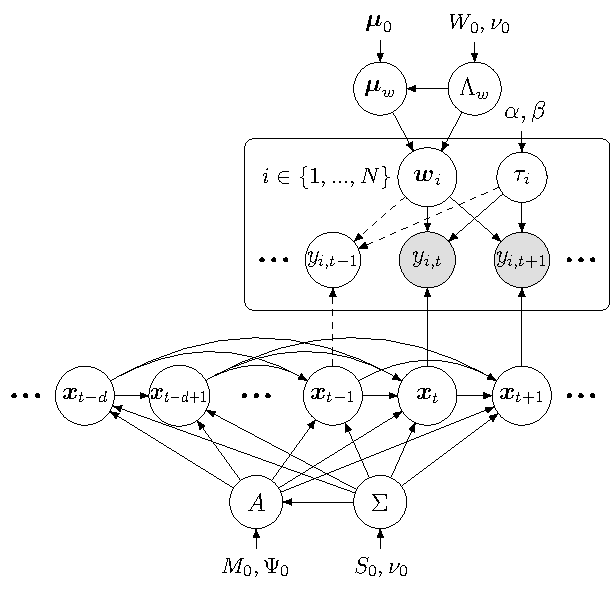
\includegraphics[scale=0.6]{graphics/btmf_net.pdf}
\end{center}
\scriptsize
\begin{itemize}
    \item[\color{black}\textbullet] Graphical model of BTMF (time lag set: $\{1,2,\ldots,d\}$). The shaded node $(y_{i,t})$ are the observed data in $\Omega$.
\end{itemize}
\end{frame}

\end{document}